% Set up the document
\documentclass{article}

% Page size
\usepackage[
    letterpaper,]{geometry}

% Lines between paragraphs
\setlength{\parskip}{\baselineskip}
\setlength{\parindent}{0pt}

% Math
\usepackage{mathtools}
\usepackage{amssymb}
\usepackage{amsthm}
\usepackage{commath}

% Number sets
\newcommand{\C}{\mathcal{C}}
\newcommand{\N}{\mathbb{N}}
\newcommand{\Q}{\mathbb{Q}}
\newcommand{\R}{\mathbb{R}}
\newcommand{\Z}{\mathbb{Z}}

% Links
\usepackage{hyperref}

% Page numbers at top right
\usepackage{fancyhdr}
\pagestyle{fancy}
\fancyhf{}
\fancyhead[R]{\thepage}
\renewcommand\headrulewidth{0pt}

% Graphics
\usepackage{float}
\usepackage{graphicx}
\graphicspath{ {./img/} }

% MATLAB stuff
\usepackage[numbered,framed]{matlab-prettifier}
\lstset{
  style              = Matlab-editor,
  mlshowsectionrules = true,
}

\begin{document}

\textbf{MATH 419 homework 1} \\
\textbf{Matt Wiens \#301294492} \\
\textbf{2020-06-02}

1.2. Write $a_n$ in terms of $b_n$ and $c_n$.

\textit{Solution.}
For this problem we want to show how the $a_n$ terms in
%
\begin{equation*}
    \sum_{n = - \infty}^\infty a_n e^{i n \theta}
\end{equation*}
%
relate to the $b_n$ and $c_n$ terms in
%
\begin{equation*}
    \sum_{n = 0}^\infty \sbr{b_n \sin(n \theta) + c_n \cos(n \theta)}
    .
\end{equation*}
%
To start, we'll use Euler's formula to write the first expression as
%
\begin{equation*}
    \sum_{n = - \infty}^\infty a_n \sbr{\cos(n \theta) + i \sin(n \theta)}
    .
\end{equation*}
%
Making use of the fact that $\cos$ is even and $\sin$ is odd we have that
%
\begin{equation*}
    \sum_{n = - \infty}^\infty a_n \sbr{\cos(n \theta) + i \sin(n \theta)}
    =
    a_0
    +
    \sum_{n = 1}^\infty \sbr{(a_n + a_{-n}) \cos(n \theta) + i (a_n - a_{-n}) \sin(n \theta)}
    .
\end{equation*}
%
Thus we have that, for $n = 0$, $c_0 = a_0$, and for $n \neq 0$,
%
\begin{align*}
    a_n + a_{-n} &= c_n, \\
    i (a_n - a_{-n}) &= b_n
    .
\end{align*}
%
To solve for the $n > 0$ $a_n$ coefficients, we
solve for $a_{-n}$ in the second equation we get
%
\begin{equation*}
    a_{-n} = a_n + i b_n
    ,
\end{equation*}
%
and so using the first equation we have
%
\begin{equation*}
    a_n + (a_n + i b_n) = c_n \implies a_n = \frac{c_n - i b_n}{2}
    .
\end{equation*}
%
To solve for the $n < 0$ $a_n$ coefficients we proceed similarly, first
solving for $a_n$ in the second equation:
%
\begin{equation*}
    a_{n} = a_{-n} - i b_n
    .
\end{equation*}
%
Substituting this into the first equation we obtain
%
\begin{equation*}
    (a_{-n} - i b_n) + a_{-n} = c_n \implies a_{-n} = \frac{c_n + i b_n}{2}
    .
\end{equation*}
%
Putting together our results, we have
%
\begin{equation*}
    a_n =
    \begin{dcases}
        \frac{c_{-n} + i b_{-n}}{2},&n < 0 \\
        c_0,&n = 0 \\
        \frac{c_n - i b_n}{2},&n > 0
    \end{dcases}
    .
\end{equation*}

\newpage

1.7. Verify that if $f$ is a trigonometric polynomial, then its
coefficients $\cbr{a_n}_{n \in \Z}$ are given by
%
\begin{equation*}
    a_n = \frac{1}{2 \pi} \int_{-\pi}^\pi f(\theta) e^{-i n \theta} \dif \theta
    .
\end{equation*}

\textit{Solution.} Suppose $f$ has the form
%
\begin{equation*}
    f(\theta) = \sum_{k = -N}^N a_k e^{i k \theta}
    .
\end{equation*}
%
Just as in the course textbook, we will multiply both sides of the
equation by $e^{-i n \theta}/2 \pi$, where $n \in \Z$:
%
\begin{equation*}
    \frac{1}{2 \pi} f(\theta) e^{- i n \theta} = \frac{1}{2 \pi} \sum_{k = -N}^N a_k e^{i k \theta} e^{-i n \theta}
    .
\end{equation*}
%
Next we integrate from $- \pi$ to $\pi$ with respect to $\theta$.
%
\begin{equation*}
    \frac{1}{2 \pi} \int_{- \pi}^\pi f(\theta) e^{- i n \theta} \dif \theta
    = \frac{1}{2 \pi} \int_{- \pi}^\pi \sum_{k = -N}^N a_k e^{i k \theta} e^{-i n \theta} \dif \theta
    .
\end{equation*}
%
Because the sum in the RHS of the above equation if finite, we are free
to interchange the sum and integral:
%
\begin{equation*}
    \frac{1}{2 \pi} \int_{- \pi}^\pi f(\theta) e^{- i n \theta} \dif \theta
    = \frac{1}{2 \pi} \sum_{k = -N}^N \int_{- \pi}^\pi  a_k e^{i k \theta} e^{-i n \theta} \dif \theta
    = \frac{1}{2 \pi} \sum_{k = -N}^N a_k \int_{- \pi}^\pi  e^{i k \theta} e^{-i n \theta} \dif \theta
    .
\end{equation*}
%
The integral containing only the exponential terms is clearly equal to
$2 \pi$ when $n = k$, and vanishes when $n \neq k$ because, setting $m = k - n \neq 0$,
%
\begin{equation*}
    \int_{- \pi}^{\pi} e^{i m \theta} \dif \theta
    =
    \int_{- \pi}^{\pi} \cos(m \theta) \dif \theta
    +
    i \int_{- \pi}^{\pi} \sin(m \theta) \dif \theta
    = 0 + i 0 = 0
    .
\end{equation*}
%
Thus, our last main equation reduces to
%
\begin{equation*}
    \frac{1}{2 \pi} \int_{- \pi}^\pi f(\theta) e^{- i n \theta} \dif \theta
    = \frac{1}{2 \pi} a_n 2 \pi
    = a_n
    .
\end{equation*}

\newpage

1.14. Use MATLAB to reproduce the plot of the sawtooth function in
  Figure 1.3 (of the course textbook). Then modify your MATLAB code to
  create a plot over the interval $[-3 \pi, 3 \pi)$ for the periodic
  extension of the function defined by $f(\theta) = \theta^2$ for
  $\theta \in [-\pi, \pi)$.

A replication of Figure 1.3 (from the course textbook) is shown in
Figure~\ref{fig:1-14-a}, while a figure for the periodic extension of
$f(\theta) = \theta^2$ defined on $[-\pi, \pi)$ is shown in
Figure~\ref{fig:1-14-b}. The code to generate these figures
(as requested by Paul Tupper) is shown in Listing~\ref{lst:1}.
%
\begin{figure}[ht]
    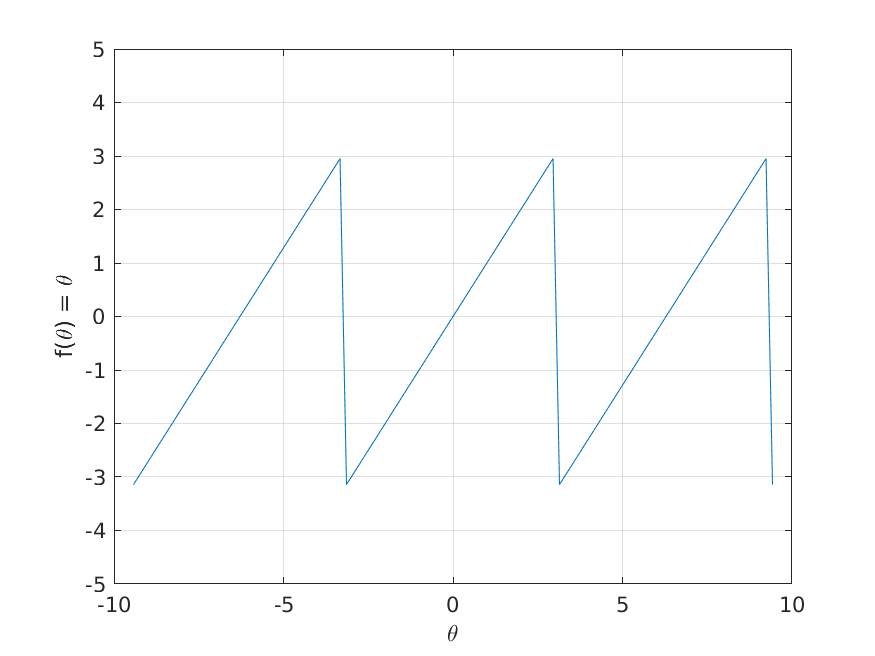
\includegraphics[width=35em]{q114a}
    \centering
    \caption{Periodic extension of $f(\theta) = \theta$ defined on $[-\pi, \pi)$}
    \label{fig:1-14-a}
\end{figure}

\begin{figure}
    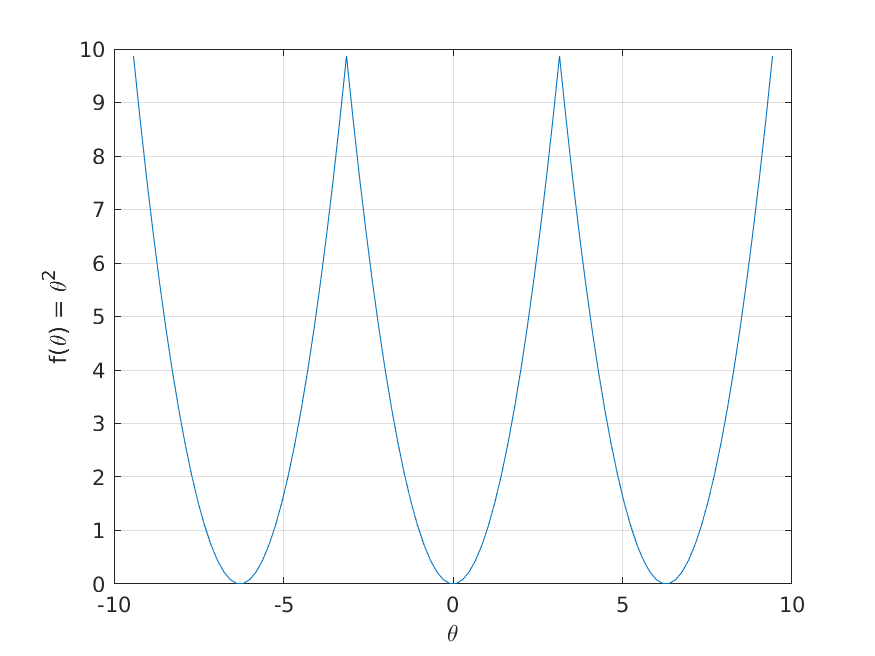
\includegraphics[width=35em]{q114b}
    \centering
    \caption{Periodic extension of $f(\theta) = \theta^2$ defined on $[-\pi, \pi)$}
    \label{fig:1-14-b}
\end{figure}

\newpage

\begin{lstlisting}[caption = {Code to generate plots},captionpos=b,label={lst:1}]
    % first figure
    xs = linspace(-3*pi, 3*pi);
    ys = mod(xs-pi, 2*pi) - pi;

    figure;
    plot(xs, ys);

    grid on;
    xlim([-10, 10]);
    ylim([-5, 5]);
    xlabel("\theta");
    ylabel("f(\theta) = \theta");

    print -dpng ../img/q114a.png

    % second figure
    xs = linspace(-3*pi, 3*pi);
    ys = (mod(xs-pi, 2*pi) - pi).^2;

    figure;
    plot(xs, ys);

    grid on;
    xlim([-10, 10]);
    ylim([0, 10]);
    xlabel("\theta");
    ylabel("f(\theta) = \theta^2");

    print -dpng ../img/q114b.png
\end{lstlisting}

\newpage

1.16. Verify that if $f$ is $2\pi$-periodic and integrable, then
%
\begin{equation*}
    \int_a^{a + 2 \pi} f(\theta) \dif \theta = \int_{-\pi}^\pi f(\theta) \dif \theta
\end{equation*}
%
for all $a \in \R$.

\textit{Solution.} Since $f$ is integrable, it has some antiderivative
$F$. We will use this fact and the fact that $f(\theta) = f(\theta + 2
\pi)$ to show that
%
\begin{equation*}
    \int_a^{a + 2 \pi} f(\theta) \dif \theta - \int_{-\pi}^\pi f(\theta) \dif \theta = 0
    .
\end{equation*}
%
We start by rewriting the LHS of the above equation as
%
\begin{equation*}
    \int_a^{a + 2 \pi} f(\theta) \dif \theta - \int_{-\pi}^\pi f(\theta) \dif \theta
    =
    \int_{-\pi + (a + \pi)}^{\pi + (a + \pi)} f(\theta) \dif \theta - \int_{-\pi}^\pi f(\theta) \dif \theta
    .
\end{equation*}
%
Making use of the antiderivative $F$ we can then write
%
\begin{equation*}
    \int_{-\pi + (a + \pi)}^{\pi + (a + \pi)} f(\theta) \dif \theta - \int_{-\pi}^\pi f(\theta) \dif \theta
    =
    \del{F(\pi + (a + \pi)) - F(-\pi + (a + \pi))}
    -
    \del{F(\pi) - F(-\pi)}
    .
\end{equation*}
%
Re-arranging terms and reverting to integrals we obtain
%
\begin{align*}
    &\del{F(\pi + (a + \pi)) - F(-\pi + (a + \pi))}
    -
    \del{F(\pi) - F(-\pi)}
    \\
    &=
    \del{F(\pi + (a + \pi)) - F(\pi)}
    -
    \del{F(- \pi + (a + \pi)) - F(-\pi)}
    \\
    &=
    \int_{\pi}^{\pi + (a + \pi)} f(\theta) \dif \theta - \int_{-\pi}^{-\pi + (a + \pi)} f(\theta) \dif \theta
    .
\end{align*}
%
Using the change of variable $z = \theta - 2 \pi$ and the fact that $f$
is $2 \pi$-periodic we can write the first integral in the last line of
the above equation as
%
\begin{align*}
    \int_{\pi}^{\pi + (a + \pi)} f(\theta) \dif \theta
    &= \int_{- \pi}^{-\pi + (a + \pi)} f(z + 2 \pi) \dif z \\
    &= \int_{- \pi}^{-\pi + (a + \pi)} f(z) \dif z
    .
\end{align*}
%
Putting together all of our steps, we thus have that
%
\begin{equation*}
    \int_a^{a + 2 \pi} f(\theta) \dif \theta - \int_{-\pi}^\pi f(\theta) \dif \theta
    =
    \int_{- \pi}^{-\pi + (a + \pi)} f(z) \dif z
    - \int_{-\pi}^{-\pi + (a + \pi)} f(\theta) \dif \theta
    = 0
    ,
\end{equation*}
%
which completes the proof.

\newpage

1.17. Verify that for each $n \in \Z$, the function
  $e^{2 \pi i n \theta / L}$ is $L$-periodic.

\textit{Solution.} Here, we need to show that
%
\begin{equation*}
    e^{2 \pi i n \theta / L} = e^{2 \pi i n (\theta + L) / L}
\end{equation*}
%
for all $\theta \in \R$. One way to derive this is through Euler's
formula (using the fact that $\sin$ and $\cos$ are $2 \pi$-periodic):
%
\begin{align*}
    e^{2 \pi i n (\theta + L) / L}
    &=
    \cos(2 \pi n (\theta + L) / L)
    + i \sin(2 \pi n (\theta + L) / L)
    \\
    &=
    \cos\del{\frac{2 \pi n \theta}{L} + 2 \pi n}
    + i \sin\del{\frac{2 \pi n \theta}{L} + 2 \pi n}
    \\
    &=
    \cos\del{\frac{2 \pi n \theta}{L}}
    + i \sin\del{\frac{2 \pi n \theta}{L}}
    \\
    &=
    e^{i (2 \pi n \theta / L)}
    \\
    &=
    e^{2 \pi i n \theta / L}
    .
\end{align*}

\newpage

1.18. Let $f$ be an $L$-periodic trigonometric polynomial of degree $M$;
  that is,
%
\begin{equation*}
    f(\theta) = \sum_{n = - M}^M a_n e^{2 \pi i n \theta / L}
    .
\end{equation*}
%
Verify that $f$ coincides with its $L$-Fourier series.

\textit{Solution.} First, let's calculate the $L$-Fourier coefficients
$\widehat{f}^L(m)$ of $f$:
%
\begin{align*}
    \widehat{f}^L(m)
    &= \frac{1}{L} \int_c^{c + L} f(\theta) e^{-2 \pi i m \theta / L} \dif \theta \\
    &= \frac{1}{L} \int_c^{c + L} \del{\sum_{n = - M}^M a_n e^{2 \pi i n \theta / L}} e^{-2 \pi i m \theta / L} \dif \theta \\
    &= \frac{1}{L} \int_c^{c + L} \sum_{n = - M}^M a_n e^{2 \pi i (n - m) \theta / L} \dif \theta \\
    &= \frac{1}{L} \sum_{n = - M}^M a_n \int_c^{c + L} e^{2 \pi i (n - m) \theta / L} \dif \theta
    ,
\end{align*}
%
where in the last line we were able to swap the sum and integral because
the sum was finite. Now, if $n = m$ then clearly
%
\begin{equation*}
    \int_c^{c + L} e^{2 \pi i (n - m) \theta / L} \dif \theta = L
    ;
\end{equation*}
%
if $n \neq m$ then setting $k = n - m \neq 0$ we have
%
\begin{align*}
    \int_c^{c + L} e^{2 \pi i k \theta / L} \dif \theta
    &=
    \int_c^{c + L} \cos\del{\frac{2 \pi k \theta}{L}} + i \sin\del{\frac{2 \pi k \theta}{L}} \dif \theta \\
    &=
    \frac{L}{2 \pi k} \eval{\sin\del{\frac{2 \pi k \theta}{L}}}_c^{c + L} - i \frac{L}{2 \pi k} \eval{\cos\del{\frac{2 \pi k \theta}{L}}}_c^{c + L} \\
    &=
    \frac{L}{2 \pi k} \del{\sin\del{\frac{2 \pi k (c + L)}{L}} - \sin\del{\frac{2 \pi k c)}{L}}}
     \\ &\quad- i \frac{L}{2 \pi k} \del{\cos\del{\frac{2 \pi k (c + L)}{L}} - \cos\del{\frac{2 \pi k c)}{L}}}
    \\
    &=
    \frac{L}{2 \pi k} \del{\sin\del{\frac{2 \pi k c}{L} + 2 \pi k} - \sin\del{\frac{2 \pi k c)}{L}}}
     \\ &\quad- i \frac{L}{2 \pi k} \del{\cos\del{\frac{2 \pi k c}{L} + 2 \pi k} - \cos\del{\frac{2 \pi k c)}{L}}}
     \\
    &= 0
    ,
\end{align*}
%
where in the last step we used the $2 \pi$-periodicity of $\sin$ and $\cos$. Hence we have that
%
\begin{equation*}
    \hat{f}^L(m)
    = \frac{1}{L} \sum_{n = - M}^M a_n \int_c^{c + L} e^{2 \pi i (n - m) \theta / L} \dif \theta
    = \frac{1}{L} a_m L
    = a_m
    .
\end{equation*}
%
Thus for the $L$-Fourier series of $f$ we have
%
\begin{equation*}
    \sum_{n = - \infty}^\infty \hat{f}^L(n) e^{2 \pi i n \theta / L}
    =
    \sum_{n = - \infty}^\infty a_n e^{2 \pi i n \theta / L}
    = f(\theta)
    .
\end{equation*}

\end{document}
